\documentclass{book}

\usepackage{titling}
\title{Particle filter}
\author{Vanpaemel Simon}
\usepackage[pdftitle={\thetitle},pdfauthor={\theauthor}]{hyperref}
\usepackage[dutch]{babel}
\usepackage[utf8]{inputenc}
\usepackage{amsmath, amssymb, amsthm, siunitx , graphicx, epstopdf}
\usepackage{tabularx}
%\usepackage{subfigure}
\usepackage{epstopdf}
\usepackage[export]{adjustbox}
\usepackage{colortbl}
\usepackage{tabularx}
\usepackage[table]{xcolor}
\usepackage{booktabs}
\usepackage{float}
\usepackage{xfrac}
\usepackage{fancyhdr}
\usepackage{mathabx}
\usepackage{caption}
\usepackage{subcaption}
\captionsetup{compatibility=false}
%\usepackage{gensymb}
\usepackage{lscape}
\usepackage{multicol}
\begin{document}
\maketitle

\chapter{Particle filter}
\section{beschrijving particle filter}
De particle filter (PF) is net als de KF een specifieke implementatie van de Bayes filter.
Het verschil tussen de KF en de PF is dat deze laatste de mogelijkheid heeft om met arbitraire kansverdelingen voor $bel(x_{t})$ te werken. De KF was immers beperkt tot het gebruik van normaalverdelingen (gausscurve). Door een arbitraire kansverdeling $bel(x_{t})$ te bemonsteren wordt een groep monsters verkregen die deze kansverdeling benaderen. In de plaats van de kansverdeling continu voor te stellen, stelt men hier de kansverdeling voor door een set monsters. Dit zorgt weliswaar voor een benadering, maar dit zorgt ervoor dat de verdeling die wordt verkregen niet-parametrisch is en er dus veel meer verdelingen kunnen worden voorgesteld.

Een monster $x_{t}^{[m]}$ ($1$ $\leqslant$ $m$ $\leqslant$ $M$), met $M$ het aantal monsters, is een bepaalde toestand waarin de robot zou kunnen verkeren op tijdstip $t$. Dit is dus een hypothese en niet de werkelijke toestand van de robot. Een toestand van de robot is bijvoorbeeld de positie waar de robot zich op dat moment bevindt.
Deze monsters kunnen gegroepeerd worden in een set 
\begin{equation}
\chi_{t} =x_{t}^{[1]}, x_{t}^{[2]},...,x_{t}^{[M]}
\end{equation}

Deze set $\chi_{t}$ wordt ook wel de particle set genoemd, waarbij een particle dus een ander benaming is voor een monster. In de tekst die volgt worden deze benamingen dan ook door elkaar gebruikt.

De kans dat een hypothese $x_{t}$ deel zal uitmaken van $\chi_{t}$ is gelinkt aan de bayes filter kansuitdrukking $bel(x_{t})$:
\begin{equation}
x_{t}^{[m]}  \sim p( x_{t} | z_{1:t}  ,  u_{1:t}) 
\end{equation}
Dit zorgt ervoor dat hoe meer particles min of meer dezelfde hypothetische toestand hebben, hoe groter de kans is dat de werkelijke toestand ongeveer die toestand zal zijn.

De particle set wordt opgebouwd op een recursieve manier, $\chi_{t}$ is gebaseerd op $\chi_{t-1}$. Het algoritme dat hiervoor instaat wordt weergegeven op figuur\ref{algoritmePF}. Dit algoritme is een speciale vorm van de PF, het is namelijk het algoritme met MCL aanpassing. Het verschil met het gewone algoritme wordt uitgelegd in sectie \ref{sampling}

\begin{figure}[H]
\centering
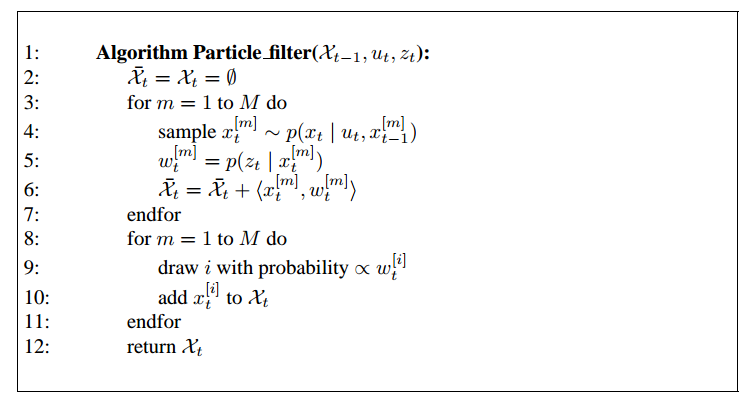
\includegraphics[width = 0.99\textwidth]{algoritmePF.png}
\caption{Algoritme voor opbouwen particle set}
\label{algoritmePF}
\end{figure}


Het algoritme genereert nieuwe mogelijke toestanden (dus nieuwe particles) voor één particle op basis van de controle signalen $u_{t}$ en de vorige hypothetische toestand van het particle (motion model). Anders gezegd neemt men de positie van het particle van de vorige tijdstap dan past men er de controlesignalen op toe en dan worden nieuwe samples gegenereerd rond deze nieuwe positie.
Daarna wordt bekeken of de nieuwe hypothetische toestand overeenkomt met de werkelijke toestand. Dit wordt verwezenlijkt door de werkelijke observatie te vergelijken met de observatie die de robot ziet indien hij zich in de hypothetische toestand bevindt. Indien deze 2 observaties overeenkomen, is het plausibel dat de nieuwe hypothetische toestand zich dicht bij de werkelijke toestand bevindt (observation model). Afhankelijk van hoe plausibel deze toestand is voor de werkelijkheid, wordt een gewicht $w_{t}^{[m]}$ gegeven aan het particle. Dit gewicht is een maat voor de belangrijkheid van het particle, als de toestand van het particle goed lijkt overeen te komen met de werkelijkheid krijgt het particle een hoog gewicht.
De particles, samen met hun gewicht, worden voorlopig opgeslaan in $\overline{\chi_{t}}$. Deze set monsters geeft eigenlijk $\overline{bel}(x_t)$ weer (prediction step).Daarna worden particles getrokken uit  $\overline{\chi_{t}}$, deze actie wordt herbemonsteren genoemd. Hoe groter het gewicht van de particles, hoe groter de kans dat de particles getrokken worden. De getrokken particles worden daarna in de definitieve particle set $\chi_{t}$ gezet. Deze particle set geeft na het herbemonsteren $bel(x_{t})$ weer (correction step), aangezien hier de observaties (gerelateerd met gewicht) worden meegenomen in de keuze van de samples.

\section{Sampling}
\label{sampling}
Aangezien de kern van de PF nu net gaat over monsters van een kansverdeling, moeten er dus bemonsterd worden om een set monsters te bekomen. Samplen van een arbitraire distributie, target distribution $f$ genoemd, is echter niet altijd mogelijk. Als oplossing wordt een andere kansverdeling bemonsterd die bemonsterbaar is, de proposal distribution $g$ genoemd. Voor deze verdeling wordt veelal de gausscurve gebruikt. Waarbij $f$ overeenkomt met $bel(x_{t})$ en $g$ overeenkomt met $\overline{bel}(x_{t})$. Door voor elk monster de kans van de target distribution te delen door de kans van de proposal distribution wordt een gewicht bekomen:

\begin{equation}
w^{[m]}=\dfrac{f(x_{[m]})}{g(x^{[m]})}
\label{gewicht}
\end{equation}

Op deze manier kan er dus worden gesampled en tegelijk een gewicht meegegeven worden aan de samples, dit wordt geïllustreerd in figuren \ref{samples1} en \ref{samples2}.
Bij MCL, een speciale vorm van de PF, wordt voor de proposal distribution het motion model gekozen. Dit is te zien op lijn vier van het algoritme op figuur\ref{algoritmePF}. Indien als proposal het motion model wordt gekozen, kan aangetoond worden dat de gewichten evenredig zijn volgens het observation model, dit is te zien op lijn vijf van het algoritme op figuur \ref{algoritmePF}. Dit laatste wordt aangetoond in sectie\ref{afleidinge}.




\begin{multicols}{2}
	\begin{figure}[H]
	\centering
	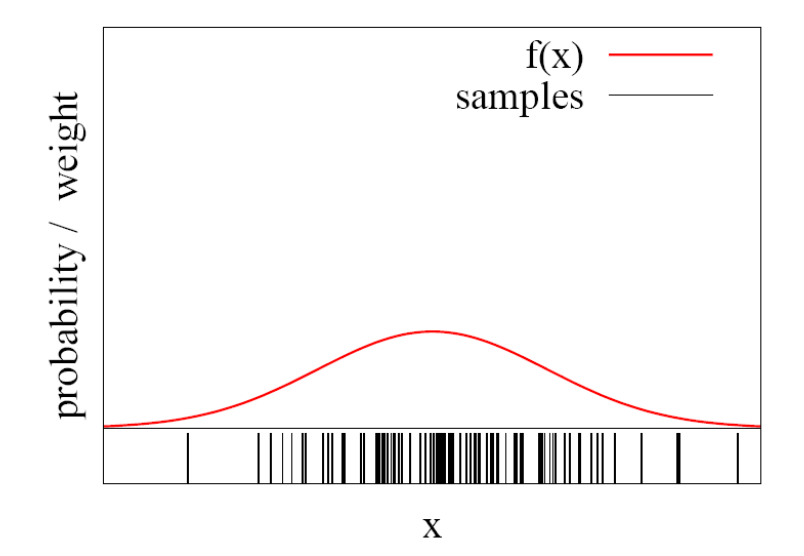
\includegraphics[width = 0.45\textwidth]{samples.png}
	\caption{Bemonstering van proposal distribution}
	\label{samples1}
	\end{figure}
	
	\begin{figure}[H]
	\centering
	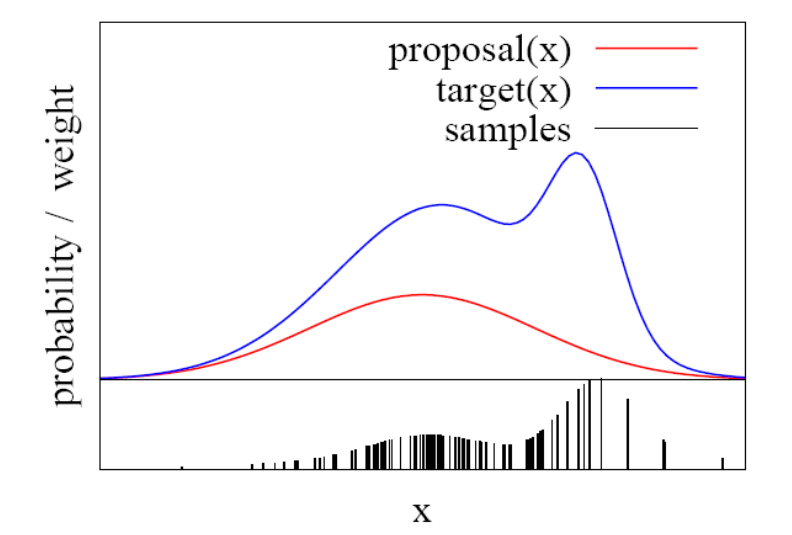
\includegraphics[width = 0.45\textwidth]{samples2.png}
	\caption{Bemonstering van target distribution}
	\label{samples2}
	\end{figure}
\end{multicols}

\section{Afleiding gewichten bij MCL particle filter}
\label{afleidinge}
In deze sectie wordt de bewering bewezen die in sectie\ref{sampling} werd gemaakt:"Indien de proposal distribution gelijk wordt genomen aan het motion model, dan de gewichten evenredig zijn met het observation model."


Ieder particle is een geschiedenis van hypothetische toestanden waarin de robot zou zijn geweest. Deze toestanden zijn, zoals bovenvermeld, in MCL de posities van de robot. Een particle bevat dus eigenlijk een hypothese van het traject dat de robot heeft doorlopen. De PF berekent dus eigenlijk $p(x_t|z_{1:t},u_{1:t})$ maar dan over alle toestanden van de robot:

\begin{equation}
bel(x_{0:t})= p(x_{0:t}| u_{1:t},z_{1:t})
\end{equation}

Analoge afleiding van sectie (JENS ZIJN AFLEIDINGE) toegepast op $bel(x_{0:t})$ levert volgende uitdrukking op (met assumptie van oneindig veel particles):
\begin{equation}
bel(x_{0:t})= p(x_{0:t}| u_{1:t},z_{1:t}) = \eta p(z_{t}|x_{t}) p(x_{t}|x_{t-1},u_{t}) p(x_{0:t-1}|z_{1:t-1},u_{1:t-1})
\label{target}
\end{equation}

Zoals bovenvermeld komt de proposal overeen met $\overline{bel}(x_{t})$, namelijk het motion model samen met een recurieve term:
\begin{equation}
\overline{bel}(x_{t})=p(x_{t}|x_{t-1},u_{t})bel(x_{0:t-1})=p(x_{t}|x_{t-1},u_{t})p(x_{0:t-1}|z_{1:t-1},u_{1:t-1})
\label{prop}
\end{equation}

vergelijkingen \ref{target} en \ref{prop} invullen in vergelijking\ref{gewicht} geeft

\begin{equation}
w_{t}^{[m]}= \dfrac{\eta p(z_{t}|x_{t}) p(x_{t}|x_{t-1},u_{t}) p(x_{0:t-1}|z_{1:t-1},u_{1:t-1})}{p(x_{t}|x_{t-1},u_{t})p(x_{0:t-1}|z_{1:t-1},u_{1:t-1})}
\end{equation}
 
met als resultaat:
\begin{equation}
w_{t}^{[m]}= \eta p(z_{t}|x_{t})
\label{gewichten}
\end{equation}

In vergelijking\ref{gewichten} zien we dat de gewichten gelijk zijn aan het observation model.
Merk op dat door te herbemonsteren met gewichten $w_{t}^{[m]}$, de overblijvende monsters in $\chi_{t}$ verdeeld zijn volgens het product van de proposal en de gewichten:
\begin{equation}
bel(x_{0:t})= \eta w_{t}^{[m]} p(x_{t}|x_{t-1},u_{t}) p(x_{0:t-1}|z_{1:t-1},u_{1:t-1})
\end{equation}


\section{Voor-en nadelen van de particle filter}
\subsection{Voordelen}
\begin{itemize}
\item Er kunnen niet-parametrische target distributions worden gebruikt.
\item Er kan geen foute data-associatie gebeuren, wat bij de KF wel kan. De reden hiervoor is dat indien de robot bijvoorbeeld 2 of meer plausibele toestanden van de werkelijkheid heeft, er tussen deze toestanden niet wordt gekozen. Ze worden immers allebei gekozen, door beide toestanden te bemonsteren. Wanneer men verdergaat in de tijd en de robot dus heeft bewogen, zullen er bepaalde toestanden minder waarschijnlijk worden en zullen deze verdwijnen. Vergelijk het met dat er op de wereld 2 exact dezelfde straten zouden zijn in een verschillende stad , dan worden deze 2 straten bemonsterd. Wanneer de robot beweegt doorheen de straat en uiteindelijk in een andere straat terechtkomt, zal in 1 van de twee straten de observatie niet overeenkomen met de map die reeds werd gemaakt, dan weet men dat men zich in de andere straat bevindt.  
\end{itemize}

\subsection{Nadelen}
\begin{itemize}
\item Er zijn veel particles nodig zodat deze monsters de gewenste target distribution goed weergeven.
\item Wanneer men bij MCL met sensoren werkt die zeer accuraat zijn ($p(z|x)$ is bijna een dirac-distributie), dan kan het zijn dat het motion model (de proposal) geen samples genereert op de plaatsen in het gebied waar $p(z|x) > 0$. Dit zorgt ervoor dat alle gewichten nul zijn, en geeft dus problemen wanneer er moet herbemonsterd worden.
\item Werkt het best als de toestandsvector laag-dimensioneel is. Aangezien een particle een hypothese is voor een toestand, zijn er minder particles nodig voor een toestand te beschrijven met een weinig aantal dimensies dan een toestand met veel dimensies. 
\label{nadelen}
\end{itemize}

\section{Mapping mbv Rao-Blackwellization}
Indien er naast de positie van de robot ook de posities van de landmarks zouden worden meegenomen in de toestandsvector, dan zou de toestandsvector hoog-dimensioneel worden. Dit is zoals gezegd in sectie \ref{nadelen} niet gewenst.
De oplossing hiervoor is om een verband te zien tussen de positie van de robot en de landmarks, namelijk eens je de positie van de robot weet, is het makkelijk om de omgeving in kaart te brengen. Want eenmaal je het traject van de robot weet, kan je de positie van de landmarks updaten met de verkregen observaties van de sensoren.
De idee is dus om met de PF de poses van de robot te bepalen. Elk sample heeft een eigen traject, en dus een eigen map die verschillend is van de andere particles. Aan ieder traject hangt dus een bepaalde map en die map is het resultaat van het traject die werd afgelegd.

Het principe van Rao-Blackwellization kan men als volgt samenvatten in formules:
\begin{equation}
p(a,b) = p(b|a) p(a)
\label{rao}
\end{equation}
Waarbij $a$ het traject van het particle voorstelt en $b$ de map voorstelt. De eerste factor $p(b|a)$ kan efficiënt berekent worden voor elk sample en p(a) stelt de samples voor, namelijk $bel(x_{0:t})$. Anders gezegd kunnen we vergelijking \ref{rao} ook voorstellen als:
\begin{equation}
p(x_{0:t},m_{1:M}|z_{1:t},u_{1:t})= p(m_{1:M}|x_{0:t},z_{1:t})p(x_{0:t}|z_{1:t},u_{1:t}) 
\end{equation}
Waarbij dus de eerste factor $p(m_{1:M}|x_{0:t},z_{1:t})$ de map opbouwd op basis van het traject en de observaties en de tweede factor $p(x_{0:t}|z_{1:t},u_{1:t})$ het traject voorstelt, merk op dat $m_{1:M}$ hier de map voorstelt op basis van landmarks, met $M$ het aantal landmarks.
Om de PF computationeel mogelijk te maken is het de bedoeling dat wanneer er een traject van het particle dus voorhanden is er efficiënt een map van dat particle kan worden opgebouwd. Alle landmarks zijn onafhankelijk van elkaar als je het traject van de robot kent (CYRILL STACHNISS ZEGT DA, LECTURE 12 minuut 20:08). Dit zorgt ervoor dat je de factor die de map met landmarks berekent kunt opsplitsen in een product dat één enkel landmark berekent. Hierbij stellen de factoren $p(m_{i}|x_{0:t},z_{1:t})$ onafhankelijke gaussische distributies voor, dit geeft:
\begin{equation}
p(x_{0:t},m_{1:M}|z_{1:t},u_{1:t})= \prod_{i=1}^Mp(m_{i}|x_{0:t},z_{1:t})p(x_{0:t}|z_{1:t},u_{1:t}) 
\end{equation}
De map wordt nog steeds gemaakt zoals in de methode van de EKF, dit komt erop neer dat er in de plaats van een hoog dimensionele EKF, moet er een kleine 2x2 EKF worden opgelost voor elk landmark. Elk particle heeft dus een 2x2 EKF dat het moet oplossen voor de bepaling van ieder landmark, wat zeer efficiënt is. De keerzijde is dat dit wel voor ieder particle moet gebeuren, maar toch is dit nog efficiënter dan indien er een hoog dimensionele EKF zou moeten worden opgelost. (DA BENK IER NIE GJIL ZEKER, zie cyrill 22:24 les 12) 

\subsection{Implementatie: FastSLAM}
\subsubsection{FastSLAM 1.0}
FastSLAM is de implementatie van de PF in combinatie met de mapping adh van Rao-Blackwellization. Hier wordt wel niet het volledige traject meegenomen maar enkel de huidige positie. Dit komt omdat wanneer de robot verder beweegt in de tijd we nooit terugkeren naar een bepaalde toestand vroeger om bijvoorbeeld de positie ervan te corrigeren. De PF kijkt altijd in de toekomst om de positie in de volgende tijdstap te berekenen. Het is de bedoeling dat er wel online, dus voor iedere tijdstap een huidige map wordt gemaakt die ergens wordt weggeschreven. Een particle houdt dus de positie bij waarop het zich op dat moment bevindt en ieder landmark wordt voorgesteld door een 2x2 EKF, zie figuur\ref{algoritmePF}.

\begin{figure}[H]
\centering
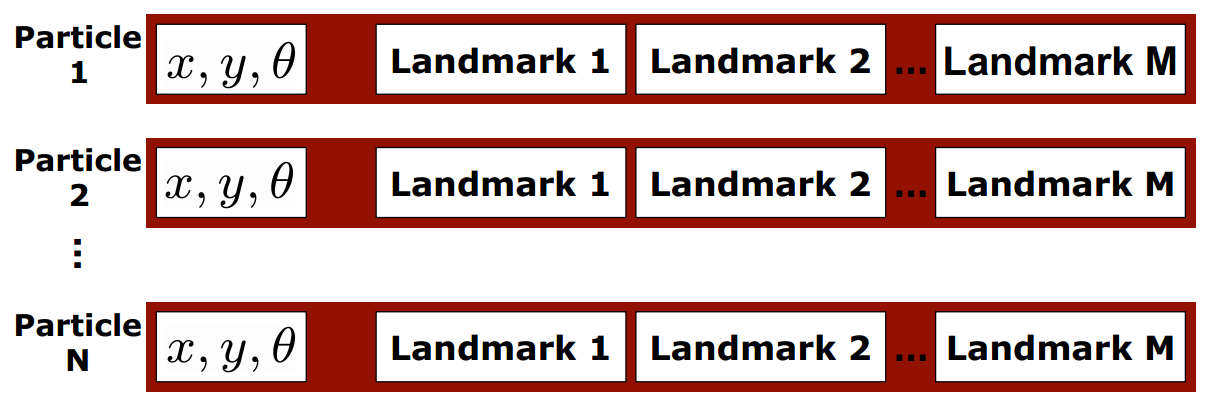
\includegraphics[width = 0.99\textwidth]{fastslam.png}
\caption{Particles bevatten hun positie en 2x2 EKF voor de voorstelling van ieder landmark}
\label{fastslam}
\end{figure}
%%FIGUUR :http://ais.informatik.uni-freiburg.de/teaching/ws13/mapping/pdf/slam12-fastslam.pdf

\subsubsection{FastSLAM 2.0}
Het verschil met Fastslam 1.0 is om in de proposal distribution niet enkel de odometry te gebruiken voor het bepalen van de volgende toestand maar nu ook rekening te houden met sensor informatie. Dit zorgt ervoor dat meer samples beter zullen aansluiten bij de target distribution. Dit zorgt er voor dat er minder particles nodig zijn en dat de map nauwkeuriger zal zijn.



\subsection{Grid-Based FastSLAM}
Dit is een particle gebaseerd SLAM algoritme voor het maken van grid-maps. Het voordeel is dat er geen feature moet worden ingebouwd om data-associatie te verwezenlijken tussen de landmarks en er dus geen foute data-associatie kan gebeuren. 
Grid-Based SLAM maakt gebruikt van het principe van FastSLAM 2.0 omdat er hier landmarks zijn waarbij de robot deze bij de measurement update kan corrigeren. Een grid map waarbij het traject niet heel correct is, is minder goed dan een landmark gebaseerde map voor navigatie.
De observatie die wordt meegenomen in de proposal distribution is een zogenaamde scan-matcher. Hierbij wordt de kans gemaximaliseerd dat deze huidige map en positie relatief overeenkomt met de vorige map en positie. Anders gezegd neemt men de map van de vorige positie en de map van de huidige positie en verschuift men (roteren,transleren) de map zodat de huidige map het best overlapt met de vorige map. In formule wordt dit als volgt weergegeven:

\begin{equation}
x_{t}^{*}=\underset{x_{t}}{argmax}\{p(z_{t}|x_{t},m_{t-1})p(x_{t}|u_{t-1},x_{t-1}^{*}) \}
\end{equation}

Mathematisch gezien is dit niet volledig correct, aangezien de observatie al reeds wordt gebruikt in de proposal distribution. Dit zorgt ervoor dat de berekening voor de gewichten zou moeten worden aangepast.
Als oplossing hiervoor wordt niet alles gescanmatched, maar enkel bepaalde blokken van bijvoorbeeld 100 posities. Als resultaat krijg je voor die 100 posities een locale map die nauwkeurig is, en dan gebruik je de scanmatcher om deze lokale mappen te laten overlappen.









\end{document}